\documentclass{article}
\usepackage{graphicx} % Required for inserting images

\title{Deffuant Model of Opinion Dynamics}
\author{Nathan Rees}
\date{September 2026}

\begin{document}

\maketitle

\section{Introduction}
Physical models of systems such as the Ising model of ferromagnetics and entropic models for system evolutions have long existed inside the realm of statistical physics. These models have been highly successful in describing macroscopic phenomena based on key insights about the microscopic nature of the physical world. Throughout the past century, many of these principles have been applied to non-physical systems. Great success has been found especially in describing economics, even having the name "econo-physics". More recently, these principles have also been applied to the study of how opinions disseminate throughout a population. This field has adopted the name of "opinion dynamics", which aim to describe how opinions (whether discrete or continuous) change throughout a population depending on how agents communicate with one another. While this report focuses on a system that may most resemble how a continuous political ideology changes throughout the system, these principles from opinion dynamics are also applicable to other social dynamics such as language and cultural dynamics and the model in this report should not be taken as definite fact on how opinions evolve.

In opinion dynamics there are many different models that one can consider. One of the simplest is the voter model. Agents in a lattice (or network for a slightly more complicated system) take one of a discrete value (typically one of two values), and agents either change or don't change their value based on a rule (typically dependent on the values of the neighbours). For example, an agent may change their value if two or more of its neighbours have a different value. While this model is fairly simple to implement, it makes many approximations and assumptions that fail to reflect its real-world inspiration. Values of agents are typically more nuanced than a simple discrete value (such as a simple "yes" or "no" to an opinionated question). Instead, one can allow for a continuity of opinion (this can be represented as a bounded interval, such as from 0 to 1 or from -1 to +1) to encapsulate agents' opinions not being binary, but only allow for agents to communicate to their neighbours a binary opinion. This is known as a CODA (continuous opinion, discrete action) model. While this better reflects its real-world inspiration, it still fails to encapsulate how agents may strongly or weakly communicate agreement or disagreement, and also how agents may not communicate at all if difference in opinion is too great.

The Deffuant model aims to implement these into opinion dynamics. Typically, analysis for this model is conducted in a network but for this report a two dimensional lattice will be used. The Deffuant model encodes agents' opinions into a bounded interval (for this report we will take this bound as being from 0 to 1). Given a random agent and a random neighbour of the agent, the two communicate via the rule

\[x_{i}(t+1) = x_{i}(t) + \mu [x_{j}(t)-x_{i}(t)]\]
\[x_{j}(t+1) = x_{j}(t) + \mu [x_{i}(t)-x_{j}(t)]\]

where $x_{i}$ is a random agent, $x_{j}$ is a random neighbour of the agent and $\mu$ is called the convergence parameter, and is based on a compromise strategy (REFERENCE). There is also an added requirement that
\[|x_{i}(t) - x_{j}(t)| <= r\]
where r is a threshold whereby agents won't communicate unless the above is satisfied.

\section{Implementation}
\subsection{Lattice Generation}
While typically one could simply generate a lattice or network at random without any weighting, it is far more interesting to be able to have different starting conditions whereby agents are more likely to be bipartisan, centralist or any other distribution one wants to test. As such, one can specify their own lattice for analysis or use the beta distribution with varying $\alpha$ and $\beta$ parameters to produce different initial lattices. Interesting beta distributions to try include the uniform distribution ($\alpha = 1$, $\beta = 1$), a more bipartisan lattice ($\alpha = 0.5$, $\beta = 0.5$) and a more centralist distribution ($\alpha = 2$, $\beta = 2$).

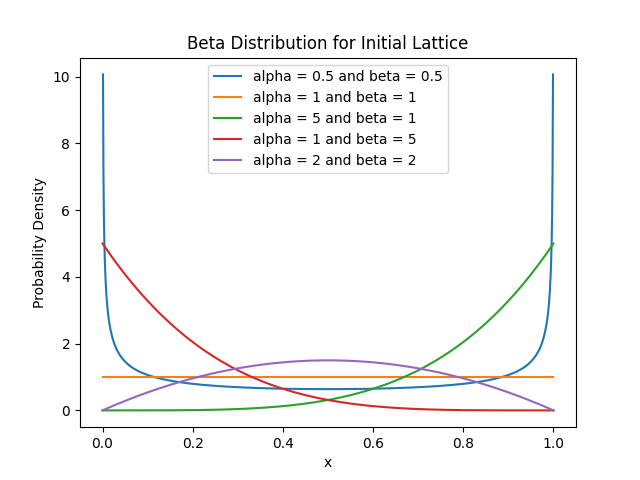
\includegraphics[width = 0.9\textwidth]{Images/Beta Distribution.png}

The code utilises numpy's random.beta function to produce a lattice of given dimensions (default 50 by 50 if no lattice is specified). An example inital voter lattice is shown below.

\begin{figure}[h]
\caption{Example of a Voter Block with $\alpha = 1$ and $\beta = 1$}
\centering
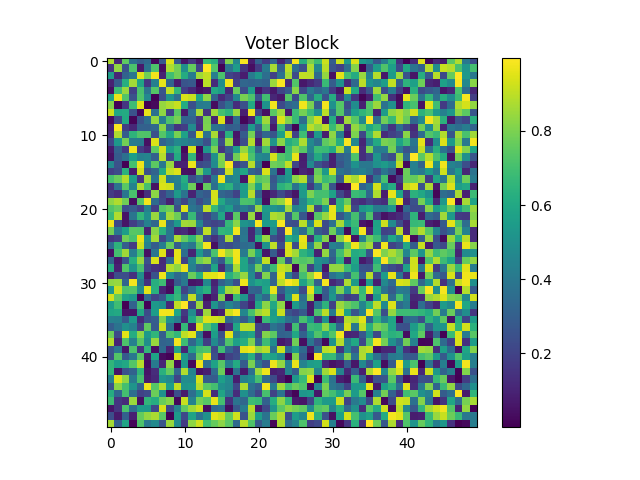
\includegraphics[width=0.9\textwidth]{Images/Example Initial Voter Block.png}
\end{figure}

The lattice generates values of 0 to 1 for each site based on the beta distribution specified. (FIG NAME HERE!!!!!!!!!) uses $\alpha = 1$ and $\beta = 1$, so every value is equally likely due to the beta distribution being a uniform distribution for these values. An example of a lattice generated with different $\alpha$ and $\beta$ is shown below.

\begin{figure}[h]
\caption{Example of a Voter Block with $\alpha = 0.5$ and $\beta = 0.5$}
\centering
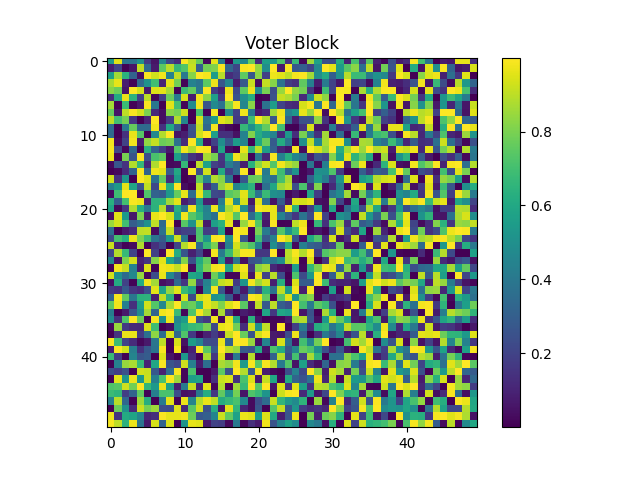
\includegraphics[width=0.9\textwidth]{Images/Example Initial Voter Block 2.png}
\end{figure}

Note how values closer to 0 and 1 are more common for a lattice where the beta distribution used to generate it has $\alpha = 0.5$ and $\beta = 0.5$ than for the lattice where $\alpha = 1$ and $\beta = 1$.

\subsection{Deffuant Model}
Two different Deffuant models were developed for the program used in this report. One model (which will be referred to as the Deffuant model) simply picks two agents at random (they do not need to be neighbours) and applies the rules laid out in the introduction, that is

\[x_{i}(t+1) = x_{i}(t) + \mu [x_{j}(t)-x_{i}(t)]\]
\[x_{j}(t+1) = x_{j}(t) + \mu [x_{i}(t)-x_{j}(t)]\]
only if 
\[|x_{i}(t) - x_{j}(t)| <= r\]
where $x_{i}$ and $x_{j}$ are two random agents (or sites) in the lattice.
The second developed model is slightly in how it chooses the two agents. An agent is chosen at random, but one of its four neighbours are chosen evenly, at random instead of a completely unrelated agent. Then the above rules are applied for updating the lattice.

A variation of the Deffuant model (which will be dubbed the noisy Deffuant model) was also developed. Instead of the threshold being a specified value, it is instead chosen from a beta distribution at random with a variable change so that a mean and variance can be specified instead of a value for $\alpha$ and $\beta$. First, $\alpha$ and $\beta$ were re-parametrised by the equations

\[\alpha = \phi \mu \quad and \quad \beta = \phi(1-\mu)\]

where $\mu$ is the mean and $\phi$ is defined as the precision. This is further re-expressed in terms of a mean and a standard deviation as to resemble a more typical normal distribution via

\[\phi = \mu\frac{1-\mu}{\sigma^{2}}-1\]

Depending on the specified model, the lattice is iterated many times to develop a new lattice. The number of iterations can be specified by the user, or instead a tolerance can be specified such that if the difference in the variance of the lattice between the latest time step and the time step that happened 4 time steps ago is less than the tolerance, the loop stops. Calculation of values such as variance is discussed later.

All models assume periodic boundaries.

Discrete voter models were also toyed with initially but these were more to test the methodology for the implementation of the Deffuant model and as such won't be discussed.

\subsection{Measurements on the System}
There are a number of metrics that were developed for to measure how the lattice evolves and to compare the three different model variations.

\subsubsection{Correlation}
The measure of "correlation" in this report is not the typical definition of correlation found in statistics. The correlation for an agent at lattice site [i,j] is defined to be
\[Correlation[i,j] = |\frac{x[i-1,j] + x[i+1,j] + x[i,j-1] + x[i,j+1]}{4} - x[i,j]|\]
 In words, the correlation for an agent is the difference between the average of the agent's neighbours and the agent. This is then averaged over all agents to find the average correlation.

 \subsubsection{Variance}
 Unlike correlation, variance has the same meaning in this report as in statistics. The lattice is squared element-by-element and then averaged using numpy, and this is subtracted from the mean of the lattice squared, as per the equation
 \[\sigma^{2} = E[X^{2}] - E[X]^{2}\]
 This is typically taken at each timestep, and is a good measure for how much the system is changing over time and hence is used to limit the number of iterations required for updating the lattice. This is done to reduce compute time.

 \subsection{Cluster Analysis}
 Some configurations of parameters result in clusters of values, and as such measurements of these clusters would be insightful. Variance and correlation may capture some of this information, but for better analysis the clusters need specific measurement and analysis tools. To do this, the lattice first has a copy made where agents now take on new values depending on the value of r (or the mean for the noisy Deffuant model). It was observed that the number of values the clusters (which will be referred to as NVC) evolved towards roughly followed the below (for $\alpha = 0.5$, $\beta = 0.5$)
 \[NVC \approx round(\frac{1}{r})-1\]
 where round is the rounding function that rounds to the nearest integer. From this, the range of values the agents can take is split evenly and agents falling into a range is given the corresponding value. For example, if r = 0.25, then $NVC = 3$ and so if an agent has value 0.85, the copy of the lattice has the agent at the same position assigned a value of 3 as it lies in range $\frac{2}{3}$ to 1. If the agent were to have value 0.51 the copy agent would be assigned value of 2 as the agent has value that lies in between $\frac{1}{3}$ and $\frac{2}{3}$. If the agent were to have value 0.16, the copy agent would have value 1 as the agent has value that lies between 0 and $\frac{1}{3}$.

 This is only applicable for r values less than 0.5 however as this starts to estimate only one or even zero clusters beyond this. As such a manual threshold was implemented such that values between 0 and 0.2 were considered in the same group, values between 0.2 and 0.4 as part of the same group, 0.4 to 0.6 as part of the same group, 0.6 to 0.8 part of the same group and 0.8 to 1 as part of the same group so that there are 5 total groups. It is worth noting that literature states that a phase transition occurs at $r=0.5$ where if $r > 0.5$ the network or lattice is expected to converge to consensus (that is network/lattice agents take practically identical values across the whole network/lattice), hence why this manual defining of group clusters is necessary beyond $r>0.5$.

 \section{Discussion}
 \subsection{Measurement Outcomes}
The $\mu$ term in the communication rule ultimately had little effect on measurement outcomes in the long term. The main effect of the $\mu$ term is that it makes the system reach its steady state at a different time scales. Typically, a $\mu$ value of around 0.5 produces the steady state quickest.

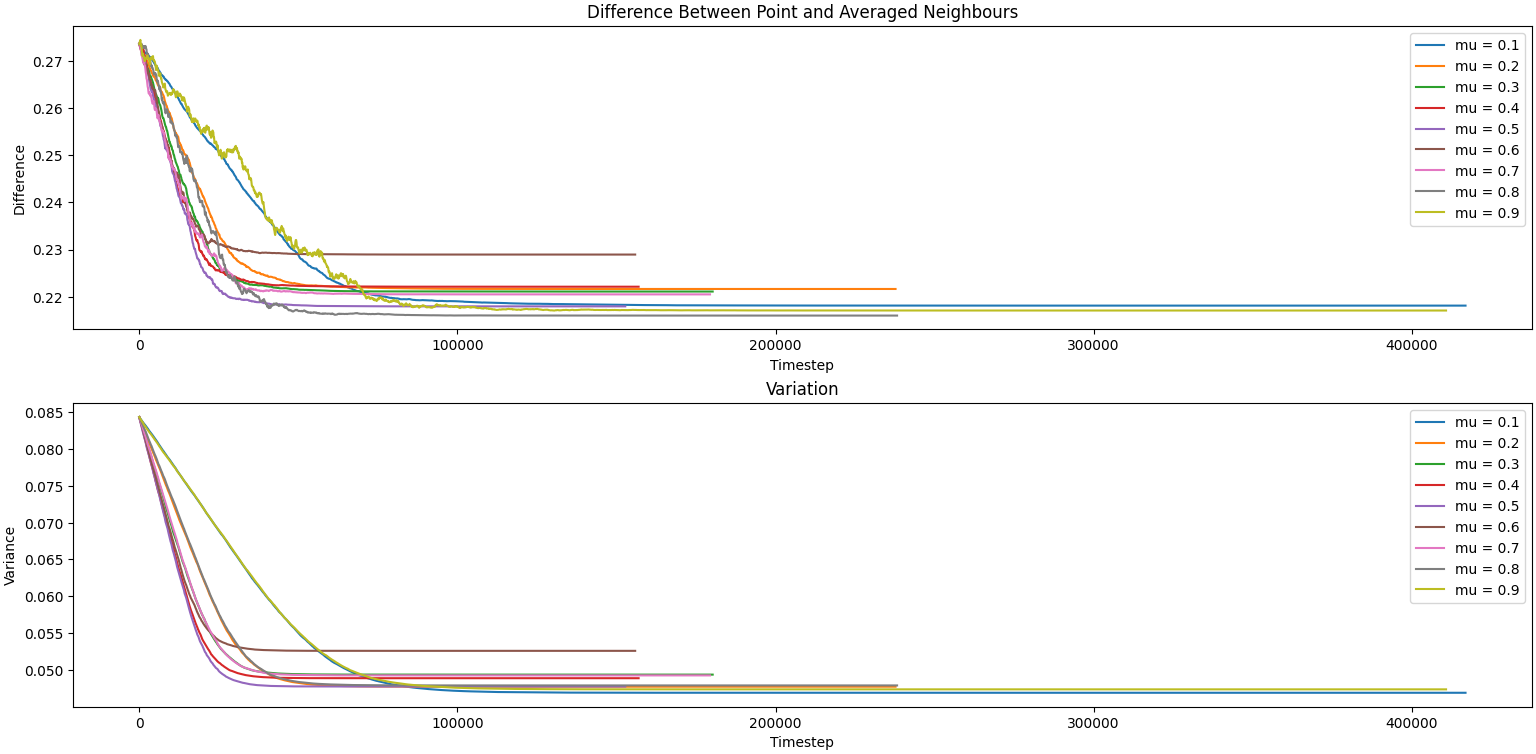
\includegraphics[width = 0.9\textwidth]{Images/diff mu values 2.png}

Another feature that doesn't affect the measurement outcomes is the dimensions of the lattice (assuming extreme values such as 1x1 or 2x2 lattices are not used). 

A $\mu$ of 0.4 is used for discussion of other behaviors such as how the r value changes the system. This is done to set a standard between different lattices and to also ensure less iterations are necessary to achieve steady state. This behavior for the $\mu$ is also reflected in the literature, it was expected to have little impact on long term iterations of the lattice and the findings of this report support  this idea.
 \subsection{Cluster Behavior}

 \subsection{Phase Transition}
 Literature states that a phase transition for a network/lattice occurs at $r=0.5$, where if $r<0.5$ the system approaches clustering behaviors and if $r>0.5$ the system approaches consensus among the agents.

\bibliography{}
https://www.ime.usp.br/~sferrari/beta.pdf
 
\end{document}
